\documentclass[compress]{beamer}
\usepackage{ifthen,verbatim}

\newcommand{\isnote}{}
\xdefinecolor{lightyellow}{rgb}{1.,1.,0.25}
\xdefinecolor{darkblue}{rgb}{0.1,0.1,0.7}

%% Uncomment this to get annotations
%% \def\notes{\addtocounter{page}{-1}
%%            \renewcommand{\isnote}{*}
%% 	   \beamertemplateshadingbackground{lightyellow}{white}
%%            \begin{frame}
%%            \frametitle{Notes for the previous page (page \insertpagenumber)}
%%            \itemize}
%% \def\endnotes{\enditemize
%% 	      \end{frame}
%%               \beamertemplateshadingbackground{white}{white}
%%               \renewcommand{\isnote}{}}

%% Uncomment this to not get annotations
\def\notes{\comment}
\def\endnotes{\endcomment}

\setbeamertemplate{navigation symbols}{}
\setbeamertemplate{headline}{\mbox{ } \hfill
\begin{minipage}{5.5 cm}
\vspace{-0.75 cm} \small
\end{minipage} \hfill
\begin{minipage}{4.5 cm}
\vspace{-0.75 cm} \small
\begin{flushright}
\ifthenelse{\equal{\insertpagenumber}{1}}{}{Jim Pivarski \hspace{0.2 cm} \insertpagenumber\isnote/\pageref{numpages}}
\end{flushright}
\end{minipage}\mbox{\hspace{0.2 cm}}\includegraphics[height=1 cm]{../cmslogo} \hspace{0.1 cm} \includegraphics[height=1 cm]{../tamulogo} \hspace{0.01 cm} \vspace{-1.05 cm}}

\begin{document}
\begin{frame}
\vfill
\begin{center}
\textcolor{darkblue}{\Large Beam-Halo Alignment}

\vfill
\begin{columns}
\column{0.6\linewidth}
\begin{center}
\large
Jim Pivarski, Alexei Safonov, Aysen Tatarinov, Vadim Khotilovich
\end{center}
\end{columns}

\begin{columns}
\column{0.3\linewidth}
\begin{center}
\scriptsize
{\it Texas A\&M University}
\end{center}
\end{columns}

\vfill
15 March, 2010

\end{center}
\end{frame}

%% \begin{notes}
%% \item This is the annotated version of my talk.
%% \item If you want the version that I am presenting, download the one
%% labeled ``slides'' on Indico (or just ignore these yellow pages).
%% \item The annotated version is provided for extra detail and a written
%% record of comments that I intend to make orally.
%% \item Yellow notes refer to the content on the {\it previous} page.
%% \item All other slides are identical for the two versions.
%% \end{notes}

\small

\begin{frame}
\frametitle{Outline}
\begin{itemize}\setlength{\itemsep}{0.5 cm}
\item Analysis of beam halo data, missing chambers

\item Closure constraint

\item Alignment results, compared with photogrammetry

\item Resolution versus integrated luminosity projections

\item Infrastructure developments

\end{itemize}
\end{frame}

\begin{frame}
\frametitle{Beam-halo data!}

\begin{itemize}
\item About 1 million events in 40 minutes
\item Distribution of beam-halo used in CSC-Overlaps alignment
\end{itemize}

\begin{columns}
\column{0.64\linewidth}
\includegraphics[width=\linewidth]{allstations.pdf}

\column{0.36\linewidth}
\includegraphics[width=\linewidth]{beamhalo2009_drdz.pdf}

\includegraphics[width=\linewidth]{beamhalo2010_drdz.pdf}
\end{columns}
\end{frame}

\begin{frame}
\frametitle{In more detail\ldots}

\begin{columns}
\column{0.7\linewidth}
\includegraphics[width=\linewidth]{xypos.png}

\column{0.3\linewidth}
\begin{itemize}
\item Divided up by station
\item Some overlaps are missing
\end{itemize}
\end{columns}

\begin{columns}
\column{0.3\linewidth}
\begin{itemize}
\item $R$ vs.\ $\phi$
\item Innermost radius set by track-reconstruction requirements
\end{itemize}

\column{0.7\linewidth}
\includegraphics[width=\linewidth]{rphipos.png}
\end{columns}
\end{frame}

\begin{frame}
\frametitle{Missing overlaps}

\only<1>{\includegraphics[width=\linewidth]{occupancy.pdf}}
\only<2>{\includegraphics[width=\linewidth]{occupancy_problems.pdf}}

\begin{itemize}
\item 4 complete rings, 6 ``almost complete'' rings, out of 15
\begin{itemize}
\item ``almost'': only one gap, which we can fill by {\it assuming} closure
\end{itemize}

\item<2> Most of the problems are edge CFEBs (1 or 5)
\end{itemize}
\end{frame}

\begin{frame}
\frametitle{Closure consistency check}

\begin{itemize}\setlength{\itemsep}{0.25 cm}
\item Closure per chamber = $\displaystyle \frac{1}{N} \sum_i^{N} \Delta (r\phi)_i - \Delta (r\phi)_{i+1}$ \hfill $N=18$ or $36$
\begin{itemize}
\item independent of alignment
\item can only be computed for complete rings
\item non-zero value interferes with alignment of incomplete rings
\end{itemize}
\end{itemize}

\vfill
\begin{columns}
\column{0.7\linewidth}
\begin{tabular}{c c c}
\hline\hline
& \hspace{0.25 cm}2008\hspace{0.25 cm} & \hspace{0.25 cm}2010\hspace{0.25 cm} \\\hline
ME$+$3/1 &                       & $+$298 $\pm$ 9~$\mu$m \\
ME$-$2/1 & $-$40 $\pm$ 23~$\mu$m & \\
ME$-$3/1 & $-$20 $\pm$ 28~$\mu$m & $+$486 $\pm$ 9~$\mu$m \\
ME$-$3/2 &                       & $+$572 $\pm$ 27~$\mu$m \\
ME$-$4/1 &                       & $+$440 $\pm$ 10~$\mu$m \\\hline\hline
\end{tabular}
\column{0.3\linewidth}
\includegraphics[width=\linewidth]{residuals2.pdf}
\end{columns}

\begin{itemize}
\item Strip-width effect in 2008 (before correction): 800~$\mu$m
\end{itemize}
\end{frame}

\begin{frame}
\frametitle{Hypothesis \#1: curving tracks}

\begin{itemize}
\item What's different between the 2008 and 2010 data?  Magnetic field

\item Radial component of magnetic field can affect beam-halo, parallel with the beamline; field is significantly radial in endcap

\item In the algorithm, tracks are assumed to propagate linearly (over
  a 10's of cm distance through gas volume)

\item Perhaps we're seeing a bias from curving tracks?
\end{itemize}

\vfill
\begin{itemize}
\item No.  Select straight $|p| > 100$~GeV tracks

\item No significant effect on closure:

\vfill
\begin{tabular}{c c c c}
\hline\hline
& 2008 (no field) & 2010, all momenta & $|p| > 100$~GeV \\\hline
ME$+$3/1 &                       & $+$298 $\pm$ 9~$\mu$m & $+$188 $\pm$ 53~$\mu$m \\
ME$-$3/1 & $-$20 $\pm$ 28~$\mu$m & $+$486 $\pm$ 9~$\mu$m & $+$483 $\pm$ 50~$\mu$m \\\hline\hline
\end{tabular}
\end{itemize}
\end{frame}

\begin{frame}
\frametitle{Hypothesis \#2: curving disks}

\begin{columns}
\column{0.4\linewidth}
\includegraphics[width=\linewidth]{bowing.pdf}

\column{0.6\linewidth}

\vspace{2 cm}
\begin{itemize}
\item $\Delta \mbox{circumference} = N \cdot \mbox{closure-per-chamber} = 2\pi \, \Delta \mbox{radius}$

\item Should try realistic disk-bending simulation from Oleg

\item With correct closure in complete rings, we can align ``almost
  complete'' rings by assuming closure = zero, but it wouldn't be valid now

\end{itemize}
\end{columns}
\end{frame}

\begin{frame}
\frametitle{Inner ring results}

\begin{itemize}
\item Complete rings only
\end{itemize}

\includegraphics[width=\linewidth]{compare_complete.pdf}
\end{frame}

\begin{frame}
\frametitle{First complete outer-ring}
\begin{center}
\includegraphics[width=0.9\linewidth]{compare_mem32_x.pdf}

\includegraphics[width=0.9\linewidth]{compare_mem32_phiz.pdf}
\end{center}
\end{frame}

%% ME+2/1 almost complete
%% ME+3/1 complete: closure per chamber = 298 +- 9 microns
%% ME+3/2 almost complete
%% ME+4/1 almost complete
%% ME+4/2 almost complete
%% ME-2/1 almost complete
%% ME-2/2 almost complete
%% ME-3/1 complete: closure per chamber = 486 +- 9 microns
%% ME-3/2 complete: closure per chamber = 572 +- 27 microns
%% ME-4/1 complete: closure per chamber = 440 +- 10 microns
%% old ME-2/1 closure per chamber = -40 +- 23 microns
%% old ME-3/1 closure per chamber = -20 +- 28 microns

%% \section*{First section}
%% \begin{frame}
%% \begin{center}
%% \Huge \textcolor{blue}{First section}
%% \end{center}
%% \end{frame}

\begin{frame}
\frametitle{Connecting rings to tracker}

\begin{itemize}
\item Established technique with cosmics; completes endcap alignment with 400~$\mu$m accuracy at 5~pb$^{-1}$ if rings can be aligned internally
\end{itemize}

\begin{columns}
\column{0.55\linewidth}
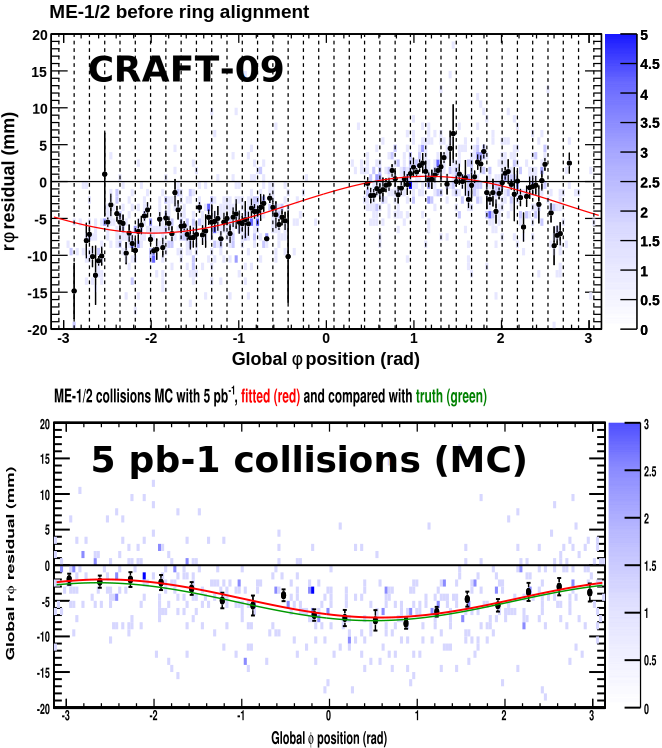
\includegraphics[width=\linewidth]{all_ringfits.pdf}
\column{0.45\linewidth}
\includegraphics[height=\linewidth, angle=90]{mccsc_diskstats_xy.pdf}

\includegraphics[height=\linewidth, angle=90]{mccsc_diskstats_phiz.pdf}
\end{columns}
\end{frame}

\begin{frame}
\frametitle{Reference-Target algorithm}

\begin{itemize}
\item Alignment of each chamber relative to the tracker individually:

does not require complete rings
\item Comparison of CSC-Overlaps against Reference-Target would be a powerful systematics check, even if only in a few rings
\item Aysen Tatarinov (TAMU) is learning the system from the inside out, and solved the problem of Minuit failing in some low-statistics fits
\end{itemize}

\mbox{ } \hfill \includegraphics[width=0.87\linewidth]{resolution_vs_intlumi.pdf} \hfill \mbox{ }
\end{frame}

\begin{frame}
\frametitle{Infrastructure developments}

\begin{itemize}
\item Alignment Quality Monitor, by Vadim Khotilovich
\item One application: server for hardware/track-based comparison plots
\end{itemize}

\begin{center}
\includegraphics[width=0.8\linewidth]{vadims_browser.png}
\end{center}
\end{frame}

\begin{frame}
\frametitle{Conclusions}

\mbox{ } \hfill \includegraphics[width=0.6\linewidth]{compare_m31_x.pdf} \hfill \mbox{ }

\begin{itemize}
\item Beam-halo run was fruitful
\begin{itemize}
\item obtained up-to-date constants for 4 rings
\item discovered a new closure issue
\item 2007 photogrammetry is still relevant
\end{itemize}

\item Next steps have all been tested in data and resolution vs.\ integrated luminosity estimated

\item New alignment group members are becoming well-versed and expanding functionality of the system
\end{itemize}

\label{numpages}
\end{frame}

\end{document}
